%%%%%%%%%%%%%%%%%%%%%%%%%%%%%%%%%%%%%%%%%%%%%%%%%%%%%%%%%%%%%%%%%%% 
%                                                                 %
%                            CHAPTER TWO                          %
%                                                                 %
%%%%%%%%%%%%%%%%%%%%%%%%%%%%%%%%%%%%%%%%%%%%%%%%%%%%%%%%%%%%%%%%%%% 
 
\chapter{Actor-Oriented Programming}\label{Actor-Oriented Programming}
SALSA is an actor-oriented programming language. This chapter starts 
first by giving a brief overview of the actor model. Section 2 
illustrates how SALSA supports the actor model.

\section{The Actor Model}\label{The Actor Model}
Actors \cite{agha-actors-86,hewitt-actors-77} provide a flexible model of concurrency for open 
distributed systems. Actors can be used to model traditional functional, 
procedural, or object oriented systems. Actors are independent, 
concurrent entities that communicate by exchanging messages 
asynchronously. Each actor encapsulates a state and a thread of 
control that manipulates this state. In response to a message, 
an actor may perform one of the following actions (see Figure~\ref{fig1}):
\begin{itemize}
\item Alter its current state, possibly changing its future behavior.
\item Send messages to other actors asynchronously.
\item Create new actors with a specified behavior.
\item Migrate to another computing host.
\end{itemize}

%begin{latexonly} 
\begin{figure}
\vspace{2.0in}
\begin{center}
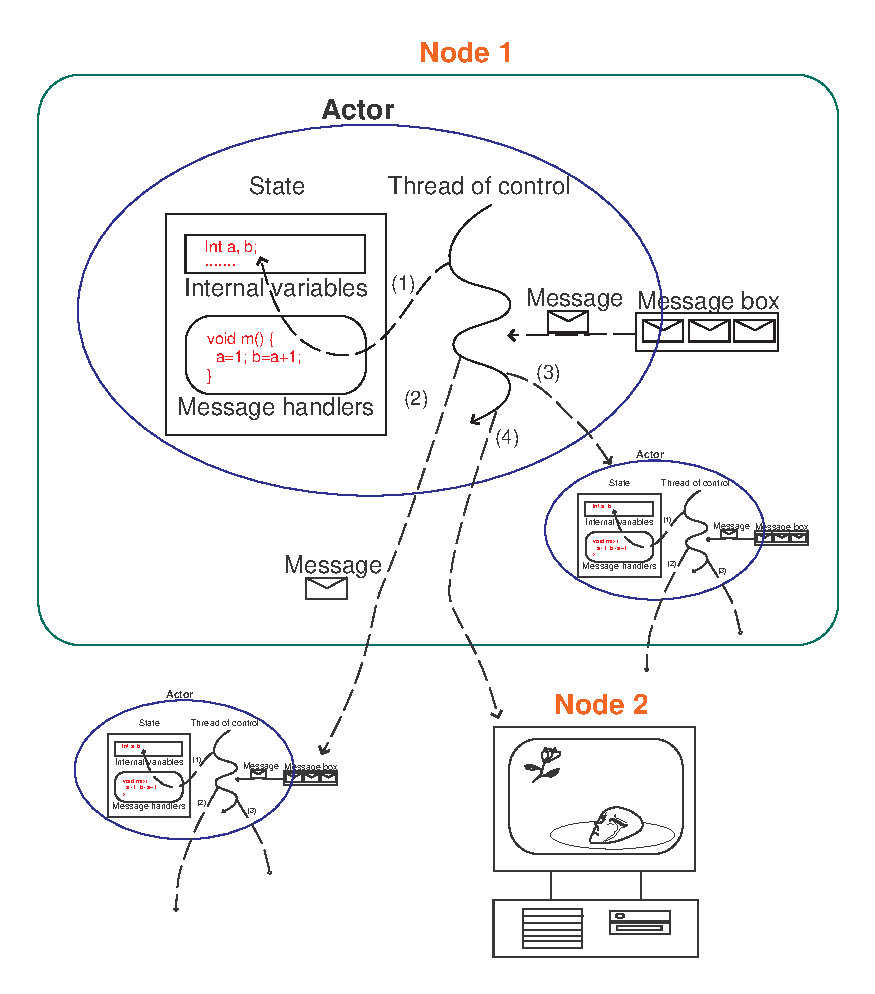
\includegraphics[angle=0,scale=0.75]{fig1.eps}
\caption{Actors are reactive entities.  In response to a message, an
actor can (1) change its internal state, 
(2) send messages to peer actors, 
(3) create new actors, 
and/or (4) migrate to another computing host.}
\label{fig1}
\end{center}
\end{figure}
%end{latexonly} 
\begin{htmlonly}
\begin{figure}
    \htmlimage{thumbnail=0.5}
    \htmlborder{5}
 \includegraphics[width=5in]{img1.png}
\caption{Actors are reactive entities.  In response to a message, an
actor can (1) change its internal state, 
(2) send messages to peer actors, 
(3) create new actors, 
and/or (4) migrate to another computing host.}
\label{fig1}
\end{figure}
\end{htmlonly}

Actors receive messages not necessarily in the same order that they 
were sent. All the received messages are initially buffered in the 
receiving actor's message box before being processed. 
Communication between actors is weakly fair: an actor infinitely 
often ready to receive a message will eventually get it. An actor can 
interact with another actor only if it has a reference to it. Actor 
references are first class entities. They can be communicated in 
messages to allow for arbitrary actor communication topologies. 
Because actors can create arbitrarily new actors, the model supports
unbounded concurrency. Furthermore, because actors only communicate
through asynchronous message passing, in particular because there is
no shared memory, actor systems are highly reconfigurable.

\section{How SALSA Supports the Actor Model}
\label{How SALSA Supports the Actor Model}
SALSA programmers write behaviors which include encapsulated state
and message handlers for actor instances:
\begin{itemize}
\item New actors get created in SALSA by instantiating particular
behaviors (with the {\tt new} keyword). Creating an actor returns
its reference.
\item The message sending operator ({\tt {\textless}-}) is used to send
messages to actors; messages contain a name that refers to the
message handler for the message and optionally a list of arguments.
\item Actors, once created, process incoming messages, one at a time. 
\end{itemize}

\section{Beyond the Actor Model}\label{Beyond the Actor Model}
While SALSA supports the actor model, it goes further in providing
linguistic abstractions for common coordination patterns in concurrent
and distributed applications. For concurrency, it provides token passing
continuations, join blocks, first-class continuations, named
tokens, and message properties. For distribution, it provides universal
naming abstractions, location-transparent remote communication, and
migration support. Furthermore, SALSA provides automatic local and
distributed garbage collection.

 
